\section{GM-3. Diseño UML del dominio y relación con LibGDX}

\subsection*{Problema}
La ampliación agrega campaña, perfil, variantes de objetos y un jefe. Sin un mapa de responsabilidades sería difícil identificar qué clase contiene cada regla.

\subsection*{Contexto}
El módulo \texttt{core} comparte el juego entre launchers. \texttt{GameLluvia} extiende \texttt{ApplicationAdapter}; \texttt{VistaJuego} utiliza los recursos gráficos y las reglas utilizan rectángulos para colisionar.

\subsection*{Solución y aplicación}
Los diagramas muestran atributos, operaciones y relaciones principales: una partida contiene personaje y lluvia; el versus contiene dos partidas; el perfil utiliza preferencias; los controles implementan una interfaz. Una flecha discontinua sin triángulo indica dependencia de uso; con triángulo hacia una interfaz indica que la clase la implementa. La herencia de clases usa línea continua y triángulo. La primera vista reúne las reglas de la partida y las abstracciones de gotas y controles. La segunda muestra perfil, dibujo, versus y jefe. Se seleccionan los miembros que explican cada responsabilidad; los métodos auxiliares y la clase heredada \texttt{GotaMala} no se incluyen. Los símbolos $+$, $-$ y $\#$ representan acceso público, privado y protegido. El rombo se coloca en la clase que contiene a las otras; el triángulo apunta a la clase o interfaz base.

\subsection*{Evidencia}
\begin{itemize}
\item \href{https://github.com/maverick1006/Proyecto-Game-LLuvia-/blob/entrega-final/core/src/main/java/puppy/code/GameLluvia.java#L14}{GameLluvia.java, línea 14} (\texttt{extends ApplicationAdapter})
\item \href{https://github.com/maverick1006/Proyecto-Game-LLuvia-/blob/entrega-final/core/src/main/java/puppy/code/Partida.java#L8}{Partida.java, línea 8} (\texttt{private final Personaje})
\item \href{https://github.com/maverick1006/Proyecto-Game-LLuvia-/blob/entrega-final/core/src/main/java/puppy/code/PartidaVersus.java#L4}{PartidaVersus.java, línea 4} (\texttt{private final Partida})
\item \href{https://github.com/maverick1006/Proyecto-Game-LLuvia-/blob/entrega-final/core/src/main/java/puppy/code/VistaJuego.java#L14}{VistaJuego.java, línea 14} (\texttt{private final SpriteBatch})
\item \href{https://github.com/maverick1006/Proyecto-Game-LLuvia-/blob/entrega-final/core/src/main/java/puppy/code/PerfilJugador.java#L9}{PerfilJugador.java, línea 9} (\texttt{private final Preferences})
\end{itemize}

\begin{figure}[htbp]
\centering
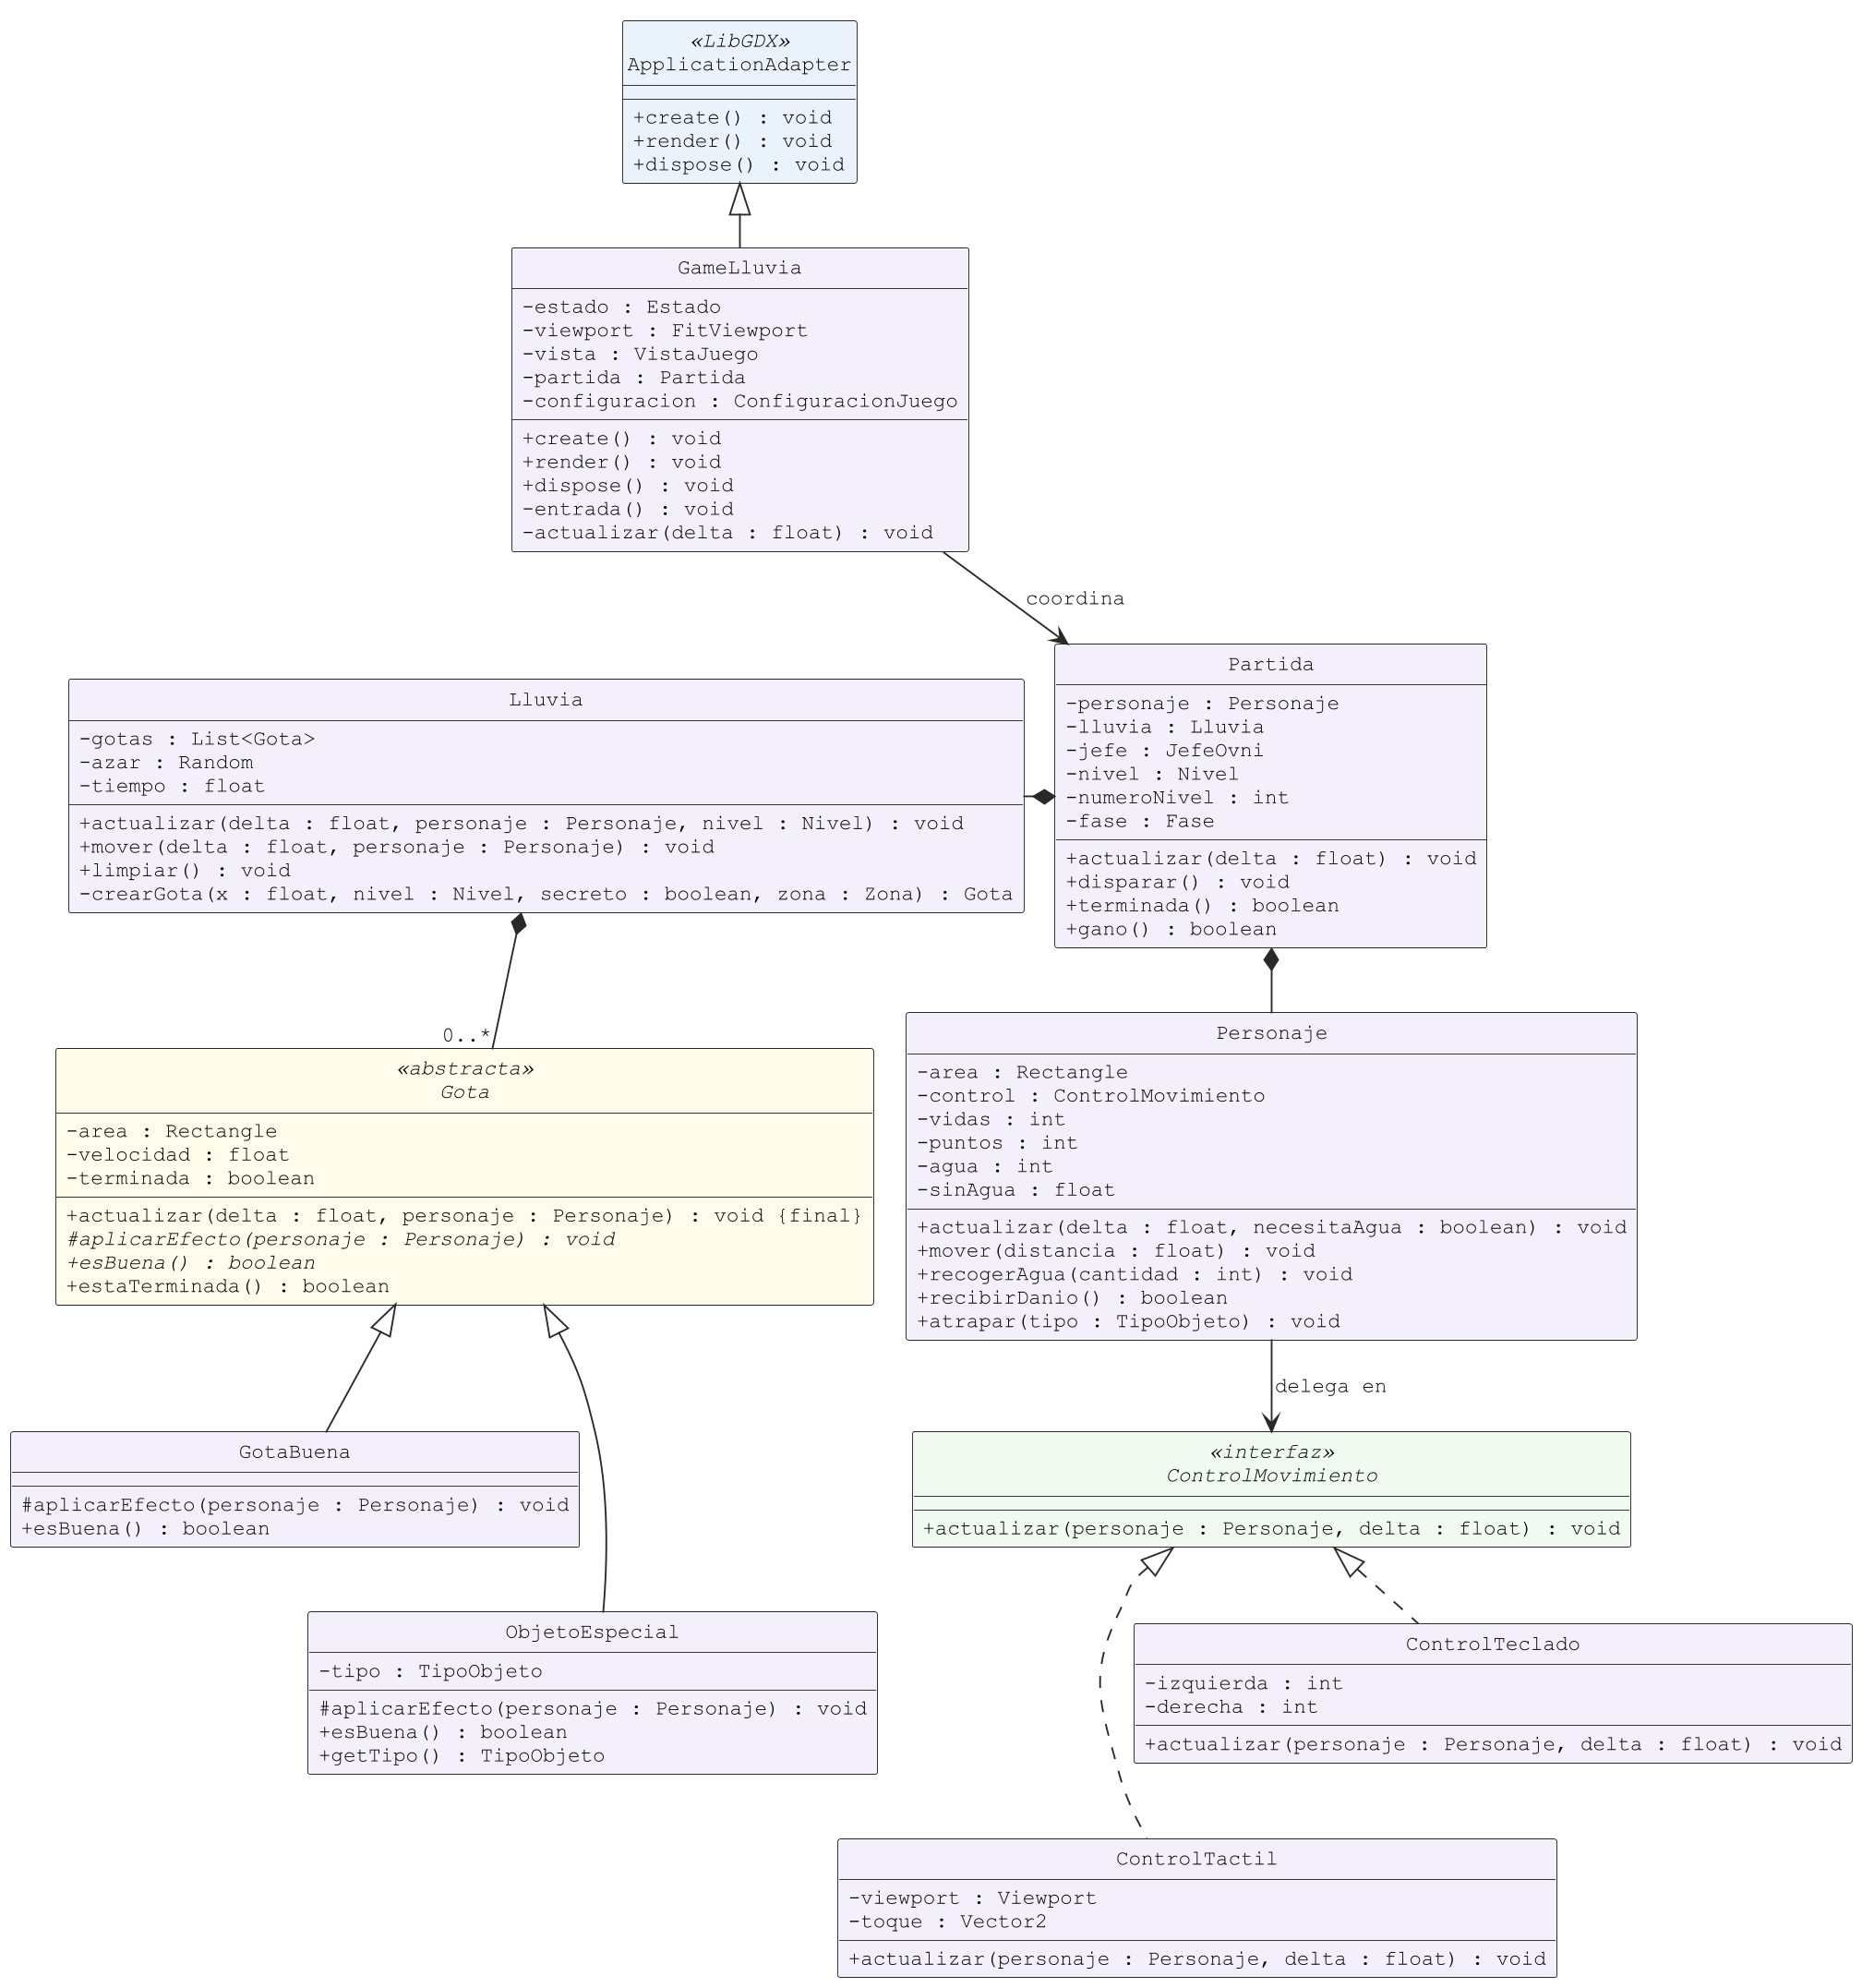
\includegraphics[width=0.95\linewidth,height=0.84\textheight,keepaspectratio]{images/01-dominio.png}
\caption{Partida, gotas y controles: atributos, métodos y relaciones}
\end{figure}





\clearpage
\begin{figure}[p]
\centering
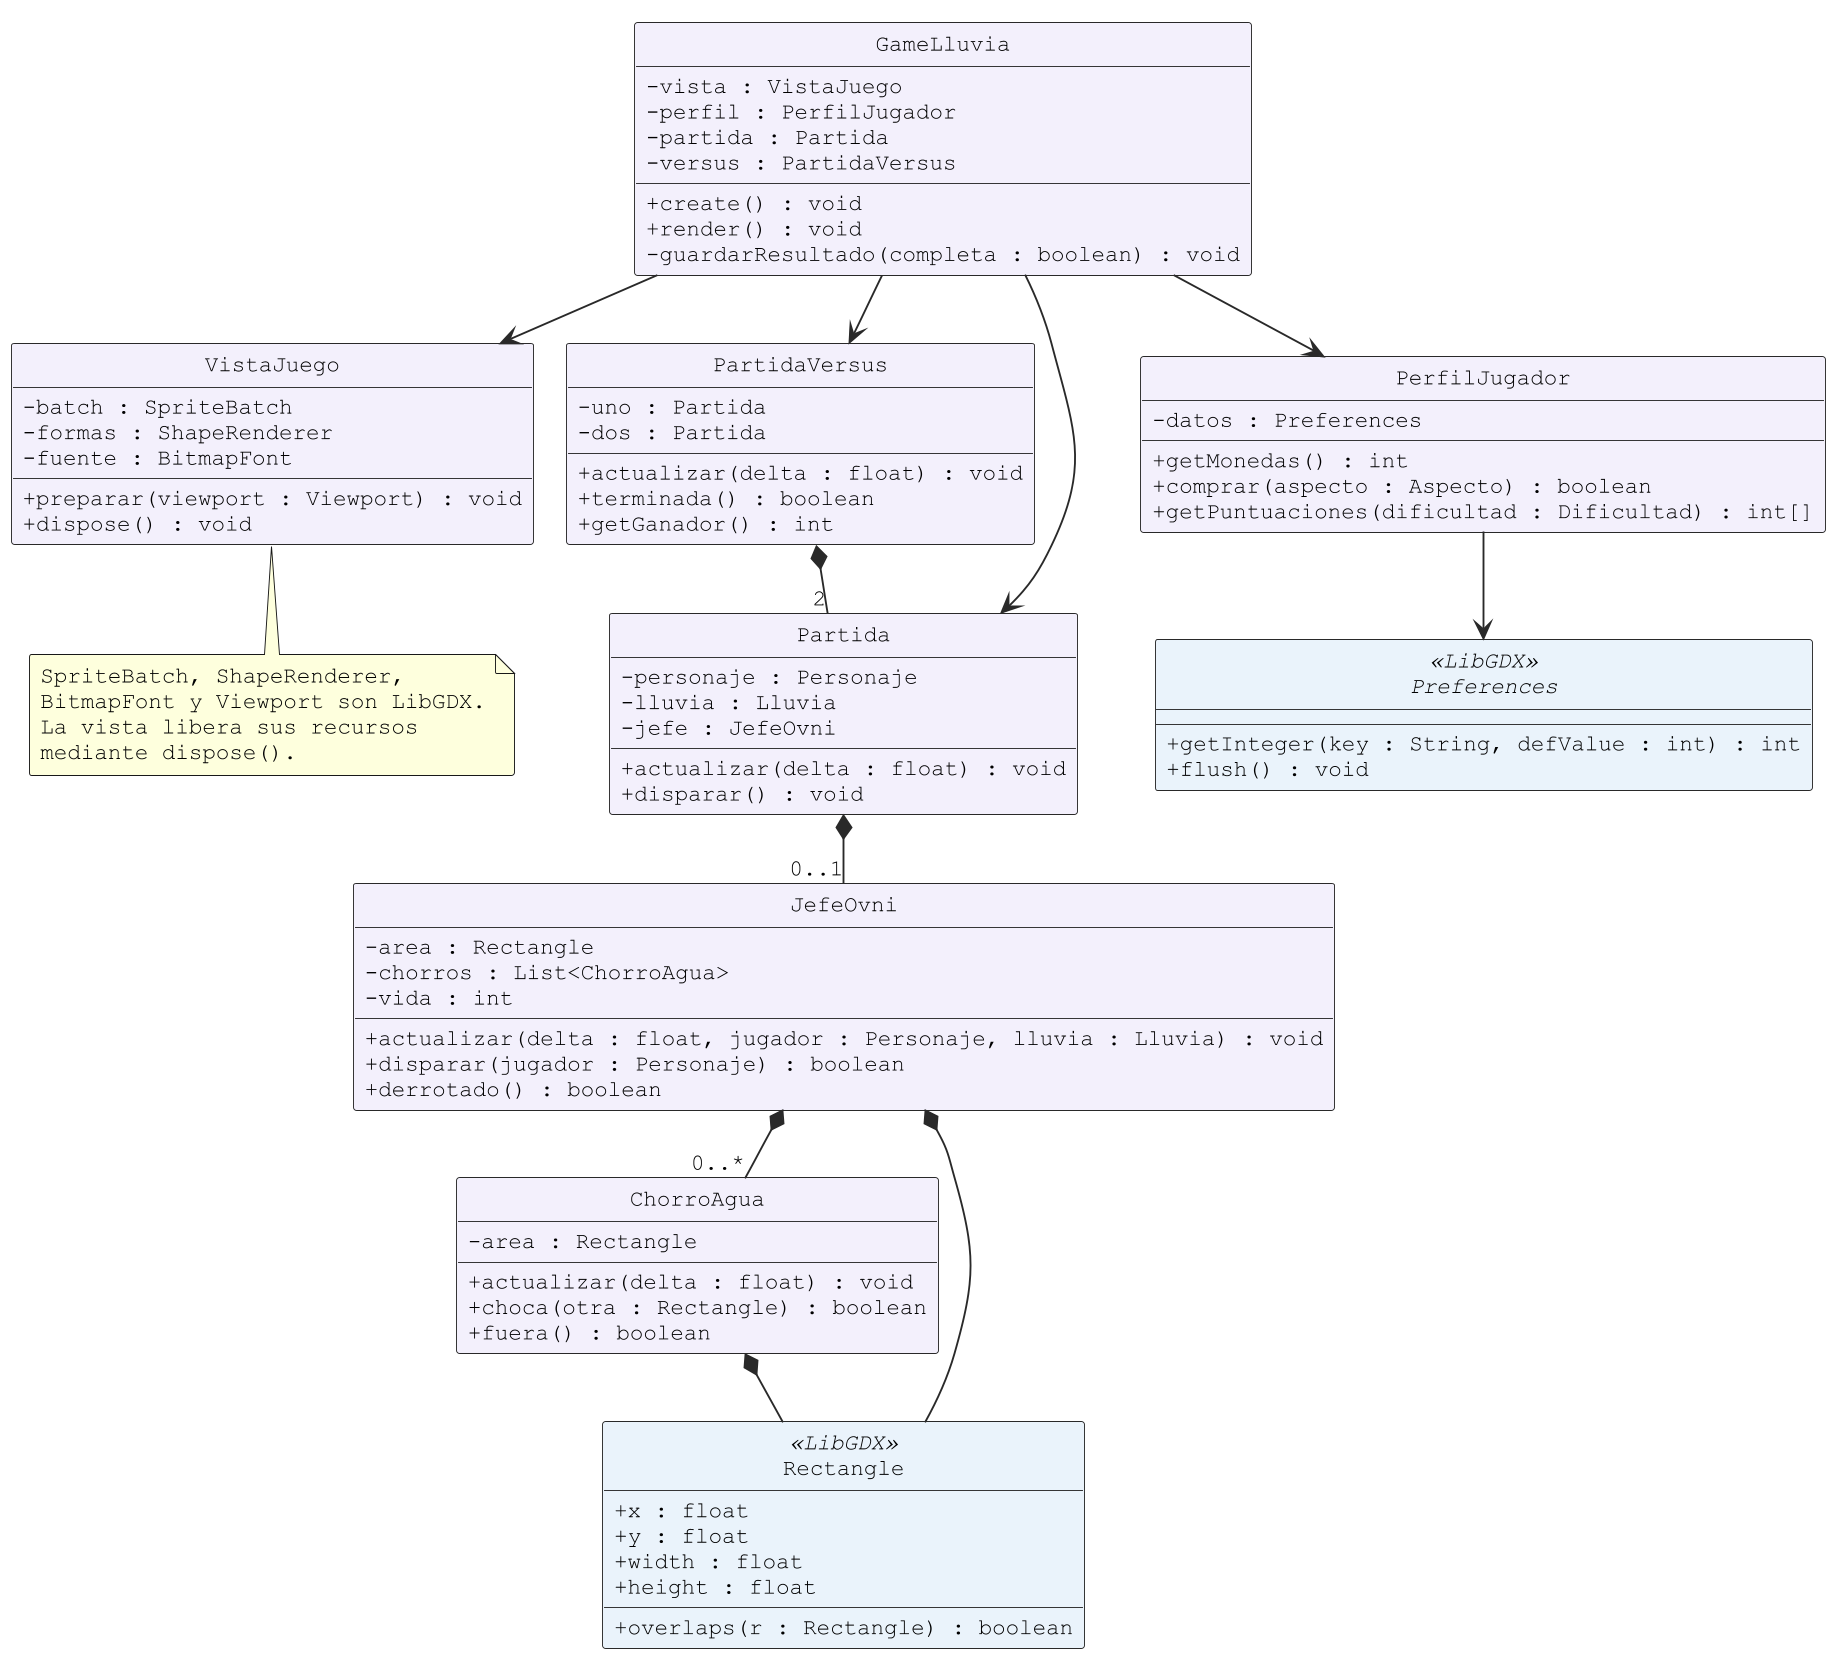
\includegraphics[width=\linewidth,height=0.84\textheight,keepaspectratio]{images/06-sistemas.png}
\caption{Perfil, presentación, versus y combate con clases de LibGDX}
\end{figure}
\clearpage
